\documentclass[a4paper,11pt]{report}
\usepackage{chuan_math_gkt}
\usetikzlibrary{angles,quotes,intersections,patterns,decorations.pathreplacing}
\chuanexamsetup

\begin{document}
\examfontsize

\examsecret{绝密$\bigstar$启用前}

\examtitle{2024年普通高等学校招生全国统一考试（天津卷）}{数\quad 学}

\noticetitle
\begin{examnotice}
\item 答卷前，考生务必将自己的姓名、准考证号填写在答题卡上. 
\item 回答选择题时，选出每小题的答案后，用铅笔把答题卡上对应题目的答案标号涂黑. 如需改动，用橡皮擦干净后，再选涂其他答案标号. 回答非选择题时，将答案写在答题卡上. 写在本试卷上无效. 
\item 考试结束后，将本试卷和答题卡一并交回. 
\end{examnotice}

\examsection{一、选择题：本大题共9小题，每小题5分，共45分. 在每小题给出的四个选项中，只有一项是符合题目要求的. }
\begin{examquestions}

\item 集合 $A=\{1,2,3,4\}$，$B=\{2,3,4,5\}$，则 $A\cap B=$
\fourchoices{$\{1,2,3,4\}$}{$\{2,3,4\}$}{$\{2,4\}$}{$\{1\}$}

\item 设 $a,b\in\mathbb R$，则“$a^3=b^3$”是“$3^a=3^b$”
\twochoices{充分不必要条件}{必要不充分条件}{充要条件}{既不充分也不必要条件}

\item 下列图中，相关性系数最大的是
\graphchoices
{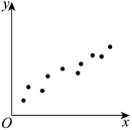
\includegraphics[width=3.0cm]{figures/2024_tj_q3_A.png}}
{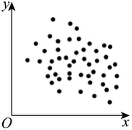
\includegraphics[width=3.0cm]{figures/2024_tj_q3_B.png}}
{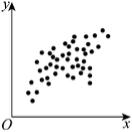
\includegraphics[width=3.0cm]{figures/2024_tj_q3_C.png}}
{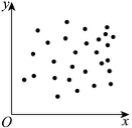
\includegraphics[width=3.0cm]{figures/2024_tj_q3_D.png}}

\item 下列函数是偶函数的是
\fourchoices{\tallchoice{$y=\dfrac{e^x-x^2}{x^2+1}$}}{\tallchoice{$y=\dfrac{\cos x+x^2}{x^2+1}$}}{\tallchoice{$y=\dfrac{e^x-x}{x+1}$}}{\tallchoice{$y=\dfrac{\sin x+4x}{e^{|x|}}$}}

\item 若 $a=4.2^{-0.3}$，$b=4.2^{0.3}$，$c=\log_{4.2}0.2$，则 $a,b,c$ 的大小关系为
\fourchoices{$a>b>c$}{$b>a>c$}{$c>a>b$}{$b>c>a$}

\item 若 $m,n$ 为两条不同的直线，$\alpha$ 为一个平面，则下列结论中正确的是
\onechoices{若 $m\parallel\alpha$，$n\subset\alpha$，则 $m\parallel n$}{若 $m\parallel\alpha$，$n\parallel\alpha$，则 $m\parallel n$}{若 $m\parallel\alpha$，$n\perp\alpha$，则 $m\perp n$}{若 $m\parallel\alpha$，$n\perp\alpha$，则 $m$ 与 $n$ 相交}

\item 已知函数 $f(x)=\sin3\left(\omega x+\dfrac\pi3\right)(\omega>0)$ 的最小正周期为 $\pi$，则函数在 $\left[-\dfrac\pi{12},\dfrac\pi6\right]$ 的最小值是
\fourchoices{\tallchoice{$-\dfrac{\sqrt3}{2}$}}{\tallchoice{$-\dfrac32$}}{$0$}{\tallchoice{$\dfrac32$}}

\item 双曲线 $\dfrac{x^2}{a^2}-\dfrac{y^2}{b^2}=1(a>0,b>0)$ 的左、右焦点分别为 $F_1,F_2$，$P$ 是双曲线右支上一点，且直线 $PF_2$ 的斜率为 $2$. $\triangle PF_1F_2$ 是面积为 $8$ 的直角三角形，则双曲线的方程为
\fourchoices{\tallchoice{$\dfrac{x^2}{8}-\dfrac{y^2}{2}=1$}}{\tallchoice{$\dfrac{x^2}{8}-\dfrac{y^2}{4}=1$}}{\tallchoice{$\dfrac{x^2}{2}-\dfrac{y^2}{8}=1$}}{\tallchoice{$\dfrac{x^2}{4}-\dfrac{y^2}{8}=1$}}

\item 一个五面体 $ABC-DEF$. 已知 $AD\parallel BE\parallel CF$，且两两之间距离为 $1$，并已知 $AD=1$，$BE=2$，$CF=3$，则该五面体的体积为

\noindent\begin{minipage}[t]{0.64\linewidth}
\twochoices{\tallchoice{$\dfrac{\sqrt3}{6}$}}{\tallchoice{$\dfrac{3\sqrt3}{4}+\dfrac12$}}{\tallchoice{$\dfrac{\sqrt3}{2}$}}{\tallchoice{$\dfrac{3\sqrt3}{4}-\dfrac12$}}
\end{minipage}\hfill
\begin{minipage}[t]{0.26\linewidth}
\vspace{-1.8em}\centering
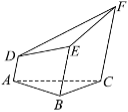
\includegraphics[width=\linewidth]{figures/2024_tj_q9.png}
\end{minipage}

\end{examquestions}

\examsection{二、填空题：本大题共6小题，每小题5分，共30分. 试题中包含两个空的，答对1个的给3分，全部答对的给5分. }
\begin{examquestions}[start=10]

\item 已知 $\mathrm{i}$ 是虚数单位，复数 $(\sqrt5+\mathrm{i})(\sqrt5-2\mathrm{i})=$\blank. 
\item 在 $\left(\dfrac3{x^3}+\dfrac{x^3}{3}\right)^6$ 展开式中，常数项为\blank. 
\item $(x-1)^2+y^2=25$ 的圆心与抛物线 $y^2=2px(p>0)$ 的焦点 $F$ 重合，$A$ 为两曲线的交点，则原点到直线 $AF$ 的距离为\blank. 
\item $A,B,C,D,E$ 五种活动，甲、乙都要选择三个活动参加. （1）甲选到 $A$ 的概率为\blank；已知乙选了 $A$ 活动，他再选择 $B$ 活动的概率为\blank. 
\newpage
\item 在边长为 $1$ 的正方形 $ABCD$ 中，点 $E$ 为线段 $CD$ 的三等分点，$\overrightarrow{CE}=\dfrac12\overrightarrow{DE}$，$\overrightarrow{BE}=\lambda\overrightarrow{BA}+\mu\overrightarrow{BC}$，则 $\lambda+\mu=$\blank；若 $F$ 为线段 $BE$ 上的动点，$G$ 为 $AF$ 中点，则 $\overrightarrow{AF}\cdot\overrightarrow{DG}$ 的最小值为\blank. 
\begin{tightcenter}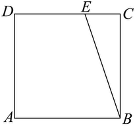
\includegraphics[width=3.0cm]{figures/2024_tj_q14.png}\end{tightcenter}
\item 若函数 $f(x)=2\sqrt{x^2-ax}-|ax-2|+1$ 有唯一零点，则 $a$ 取值范围为\blank. 

\end{examquestions}

\examsection{三、解答题：本大题共5小题，共75分. 解答应写出文字说明、证明过程或演算步骤. }
\begin{examanswers}[start=16]

\item（14分）

在 $\triangle ABC$ 中，$\cos B=\dfrac9{16}$，$b=5$，$\dfrac ac=\dfrac23$. 

\subq{（1）}{求 $a$；}

\subq{（2）}{求 $\sin A$；}

\subq{（3）}{求 $\cos(B-2A)$. }

\item（15分）

已知四棱柱 $ABCD-A_1B_1C_1D_1$ 中，底面 $ABCD$ 为梯形，$AB\parallel CD$，$A_1A\perp$ 平面 $ABCD$，$AD\perp AB$，其中 $AB=A_1A=2$，$AD=DC=1$，$N$ 是 $B_1C_1$ 的中点，$M$ 是 $DD_1$ 的中点. 

\noindent\begin{minipage}[t]{0.64\linewidth}
\subq{（1）}{求证：$D_1N\parallel$ 平面 $CB_1M$；}

\subq{（2）}{求平面 $CB_1M$ 与平面 $BB_1CC_1$ 的夹角余弦值；}

\subq{（3）}{求点 $B$ 到平面 $CB_1M$ 的距离. }
\end{minipage}\hfill
\begin{minipage}[t]{0.26\linewidth}
\vspace{-0.4em}\centering
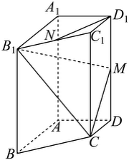
\includegraphics[width=\linewidth]{figures/2024_tj_q17.png}
\end{minipage}

\newpage
\item（15分）

已知椭圆 $\dfrac{x^2}{a^2}+\dfrac{y^2}{b^2}=1(a>b>0)$ 的离心率 $e=\dfrac12$，左顶点为 $A$，下顶点为 $B$，$C$ 是线段 $OB$ 的中点，其中 $S_{\triangle ABC}=\dfrac{3\sqrt3}{2}$. 

\subq{（1）}{求椭圆方程；}

\subq{（2）}{过点 $\left(0,-\dfrac32\right)$ 的动直线与椭圆有两个交点 $P,Q$. 在 $y$ 轴上是否存在点 $T$ 使得 $\overrightarrow{TP}\cdot\overrightarrow{TQ}\leq0$ 恒成立？若存在，求出这个 $T$ 点纵坐标的取值范围；若不存在，请说明理由. }

\item（15分）

已知数列 $\{a_n\}$ 是公比大于 $0$ 的等比数列，其前 $n$ 项和为 $S_n$. 若 $a_1=1$，$S_2=a_3-1$. 

\subq{（1）}{求数列 $\{a_n\}$ 前 $n$ 项和 $S_n$；}

\subq{（2）}{设 $b_n=\linsys{k,n=a_k,\\b_{n-1}+2k,a_k<n<a_{k+1}}$，$b_1=1$，其中 $k$ 是大于 $1$ 的正整数. }

\subq{（i）}{当 $n=a_{k+1}$ 时，求证：$b_{n-1}\geq a_k\cdot b_n$；}

\subq{（ii）}{求 $\displaystyle\sum_{i=1}^{S_n}b_i$. }

\item（16分）

设函数 $f(x)=x\ln x$. 

\subq{（1）}{求 $f(x)$ 图象上点 $(1,f(1))$ 处的切线方程；}

\subq{（2）}{若 $f(x)\geq a(x-\sqrt x)$ 在 $x\in(0,+\infty)$ 时恒成立，求 $a$ 取值范围；}

\subq{（3）}{若 $x_1,x_2\in(0,1)$，证明 $|f(x_1)-f(x_2)|\leq |x_1-x_2|^{\frac12}$. }
\end{examanswers}

\end{document}
